\documentclass[11pt]{article}

% Page geometry
\usepackage[margin=0.4in]{geometry}

% Typography
\usepackage[T1]{fontenc}
\usepackage{microtype}
\usepackage{multicol}
% Math
\usepackage{amsmath,amssymb,amsthm}

% Figures and tables
\usepackage{graphicx}
\usepackage{booktabs}
% Figures and tables
\usepackage{subcaption}
\usepackage{float}

% Make section headings smaller
\usepackage{titlesec}
% \titleformat{\section}{\normalsize\bfseries}{\thesection}{1em}{}
% \titleformat{\subsection}{\small\bfseries}{\thesubsection}{1em}{}
% \titleformat{\subsubsection}{\footnotesize\bfseries}{\thesubsubsection}{1em}{}

% % Make title smaller
% \makeatletter
% \renewcommand{\maketitle}{%
%     \begin{center}
%         {\normalsize \@title}\par
%         \vskip 0.5em
%         {\small \@author}\par
%         \vskip 0.5em
%         {\small \@date}\par
%     \end{center}
% }
% \makeatother

% Make figure and table captions smaller
% \usepackage[font=small,labelfont=bf]{caption}
% Algorithms
\usepackage{algorithm}
\usepackage{algorithmic}

% References and links
\usepackage[colorlinks=true,linkcolor=blue,citecolor=blue,urlcolor=blue]{hyperref}
\usepackage[numbers]{natbib}

% Theorem environments
\newtheorem{theorem}{Theorem}
\newtheorem{lemma}[theorem]{Lemma}
\newtheorem{proposition}[theorem]{Proposition}
\newtheorem{definition}{Definition}

% Useful shortcuts
\newcommand{\R}{\mathbb{R}}
\newcommand{\E}{\mathbb{E}}
\newcommand{\argmin}{\operatorname{argmin}}
\newcommand{\argmax}{\operatorname{argmax}}

\renewcommand{\abstractname}{Summary}

\usepackage{xcolor}

% Make blockquotes italic and gray with a line at the end
\let\oldquote\quote
\let\endoldquote\endquote
\renewenvironment{quote}{\oldquote\itshape\color{gray}}{\par\noindent\rule{\linewidth}{0.4pt}\endoldquote}


\title{The fault is in our starts and in ourselves: vision transformers for adversarial digit classification under a sparse data regime}
\author{Arjun Sharma\\
\texttt{asharma3@caltech.edu}}
\date{}

\begin{document}

\maketitle

\begin{abstract}
    This report details my attempt to train a performant Vision Transformer (ViT) over the provided `MNIST-in-the-wild' (MNIST-W) dataset. I achieve \textbf{72.9}\% validation accuracy using a model with 5.43M parameters. The model is trained on 85\% of the provided MNIST-W samples, which are passed through an aggressive data augmentation pipeline.

    A DeiT-tiny architecture, inspired by \cite{touvron2021training}, is used, with Shifted Patch Tokenization (SPT) and Locality Self Attention (LSA) \cite{lee2021vision}. These techniques, designed for sparse data regimes in previous literature, are shown in our study to improve model performance by up to 6\%, likely due to them increasing the inductive bias in the network, which is necessary in a sparse data regime.

    I include all components required by the project instructions, but swap the order of the first two parts: in \autoref{sec:data-loading}, I describe the data processing steps, particularly augmentations; in \autoref{sec:1-training-setup}, I provide a high-level overview of the basic training setup.

    My final notebook is available here: \\\href{https://colab.research.google.com/drive/1xsVW6XLaOc29qyisI_pdJXASske06-Ze?usp=sharing}{\texttt{https://colab.research.google.com/drive/1xsVW6XLaOc29qyisI\_pdJXASske06-Ze?usp=sharing}}.

\end{abstract}



% \section{Introduction}



\section{Data and preprocessing}\label{sec:data-loading}


\textbf{Data}. The provided dataset consists of 10,294 images of digits, each of which has one of 10 labels. There are $873 \pm 16$ images in each class, i.e., the difference in the number of samples is at most 3.67\% between any two classes. I therefore chose not to balance this dataset. All images are transformed to $128 \times 128$ later, as described in the dataloader implementation section.

\textbf{Split}. I chose an 85:15 train:validation split, which results in 8755 training samples and 1,539 validation samples. This split was stratified, i.e., I did not randomly selected 15\% of the entire dataset directly to generate the validation dataset; rather, for each class, I selected 15\% of the dataset to assemble the validation dataset. This ensured that the distribution of classes in the training and validation sets was as close to identical as possible.

\textbf{Augmentation}. The following augmentations are applied to every item in the training dataset, using the \texttt{transforms} module in the \texttt{TorchVision} package. 

\begin{table}[H]
\centering
\begin{tabular}{ll}
\toprule
\textbf{Transform} & \textbf{Parameters} \\
\midrule
Random resized crop & $128 \times 128$, scale $\in [0.7, 1.0]$, ratio $\in [0.75, 1.33]$ \\
Random augment & 2 operations, magnitude 9 \\
Elastic transform & $\alpha = 50.0$, $\sigma = 5.0$ \\
Gaussian blur & kernel $5\times 5$, $\sigma \sim \mathcal{U}(0.1, 2.0)$ \\
Gaussian noise & $\epsilon \sim \mathcal{N}(0, 0.05^2)$ added per pixel \\
Random erasing & $p = 0.25$, scale $\in [0.02, 0.15]$ \\
Normalization & $\mu = (0.485, 0.456, 0.406)$, $\sigma = (0.229, 0.224, 0.225)$ \\
\bottomrule
\end{tabular}
\caption{Training augmentation pipeline. Note that I needed an additional `transform' to convert the image to a PyTorch tensor before the Gaussian noise augmentation, since, up to that point, PyTorch expects a PIL image, and the last two transformations expect a tensor. Images in the validation set are passed through a different transformation pipeline: they are only resized to $128 \times 128$ and to be normalized to with the same parameters.}
\label{tab:augmentations}
\end{table}

The values for $\mu$ and $\sigma$ for the normalization steps are the values in the ImageNet dataset\footnote{Following advice I found \href{https://stackoverflow.com/questions/58151507/why-pytorch-officially-use-mean-0-485-0-456-0-406-and-std-0-229-0-224-0-2}{online}, it is acceptable to use these values for real-world images, and avoid the cost and instability of recalculating them for every training dataset -- which was helpful when I was testing different amounts of augmentations.}.

Then, for each item in the training dataset, I repeat it $N$ times per epoch with independent shuffles, where $N = 2$ for my final training run. This means every unique sample is seen $N$ times per epoch, each time with a fresh augmentation draw.


Examples of the data augmentation pipeline are presented in \autoref{fig:augmentations}.

\textbf{Dataloader implementation}. I use the PyTorch `Dataset' type. My training dataset applies the transformations in \autoref{tab:augmentations} to an image loaded from a provided path (randomly sampled from the result of the stratified split function) and returns the image and its label. The validation dataset is instantiated using the same class, but with a different set of paths provided.

A PyTorch \texttt{DataLoader} is wrapped around the combined dataset for training and the validation set. A batch size of 64 is set for both. Shuffling is set to true for training and false for validation.


\textbf{Augmentation analysis}. Augmentation encourages invariance to transformations that do not affect digit identity, and are particularly likely to be present in MNIST-W test samples. 

Given that these images were collected by different people in vastly different settings with different cameras, transformations like random resized crops and random augment operations help account for variations in framing, lighting, and camera positioning. 

The elastic transform is particularly crucial for handwritten digits, as it simulates natural variations in writing style and stroke deformation without compromising digit identity. 

To handle environmental differences across capture settings, Gaussian blur accounts for camera focus variations and motion blur, while Gaussian noise models sensor noise and varying lighting conditions. Random erasing improves robustness to partial occlusions that may occur in real-world scenarios (e.g., fingers partially covering the digit, shadows, or debris). The random resized crop parameters are set to a scale range of $[0.7, 1.0]$ and aspect ratio of $[0.75, 1.33]$ to preserve digit legibility while introducing realistic perspective variations. 

Notably, we avoid augmentations like horizontal flipping and use elastic transforms with moderate parameters ($\alpha = 50.0$, $\sigma = 5.0$) to ensure transformations remain within the manifold of valid digit representations (e.g., preventing a 6 from appearing as a 9, or a 3 from resembling an 8).

\section{Model setup}\label{sec:1-training-setup}

\textbf{Model}. More model details are in \autoref{sec:model}. My model has 3 attention heads and contains 5,427,274 parameters.

\textbf{Training}. The model was trained with cross-entropy loss \begin{equation}
    \sum_i y^{(i)} \log (p_\theta^{(i)})
\end{equation}
where $p_\theta(\cdot)$ is the output of the model. 

During the final training run, we end up taking an unusual approach to training. I trained iteratively for a few dozen epochs, pushing the ending of training closer to the deadline, and restarted training with a saved checkpoint multiple times while I felt like there was still scope to improve the performance of this model. This was an inefficient but realistic way of doing training under a deadline with sparse compute, where it was unclear from the loss history whether to dedicate additional time to improving results. This approach implicitly ended up mimicking a learning rate schedule with cold restarts until performance was saturated.

\begin{figure}[H]
  \centering
  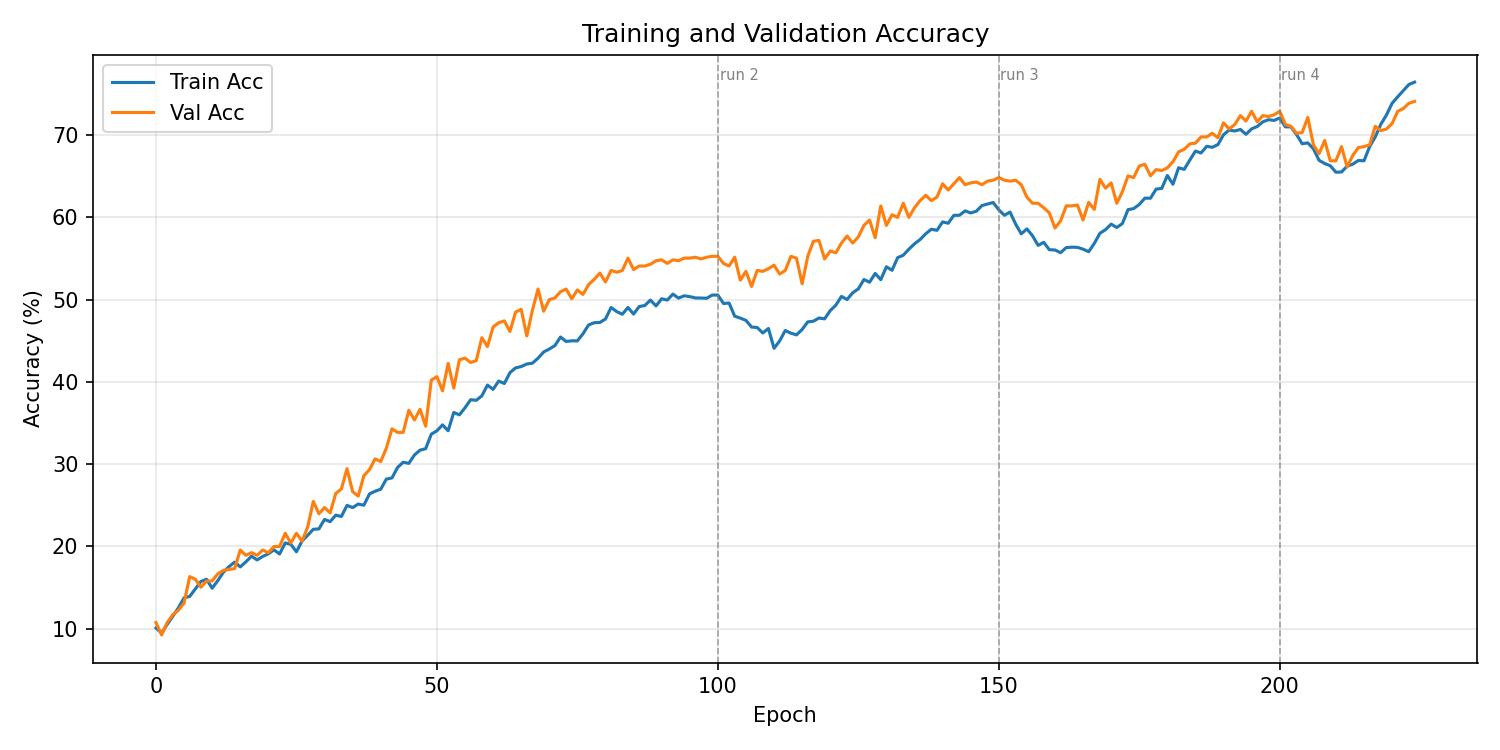
\includegraphics[width=0.5\textwidth]{figs/acc_curve.png}
  \caption{Accuracy over time with multiple restarted runs}
\end{figure}

\begin{figure}[H]
  \centering
  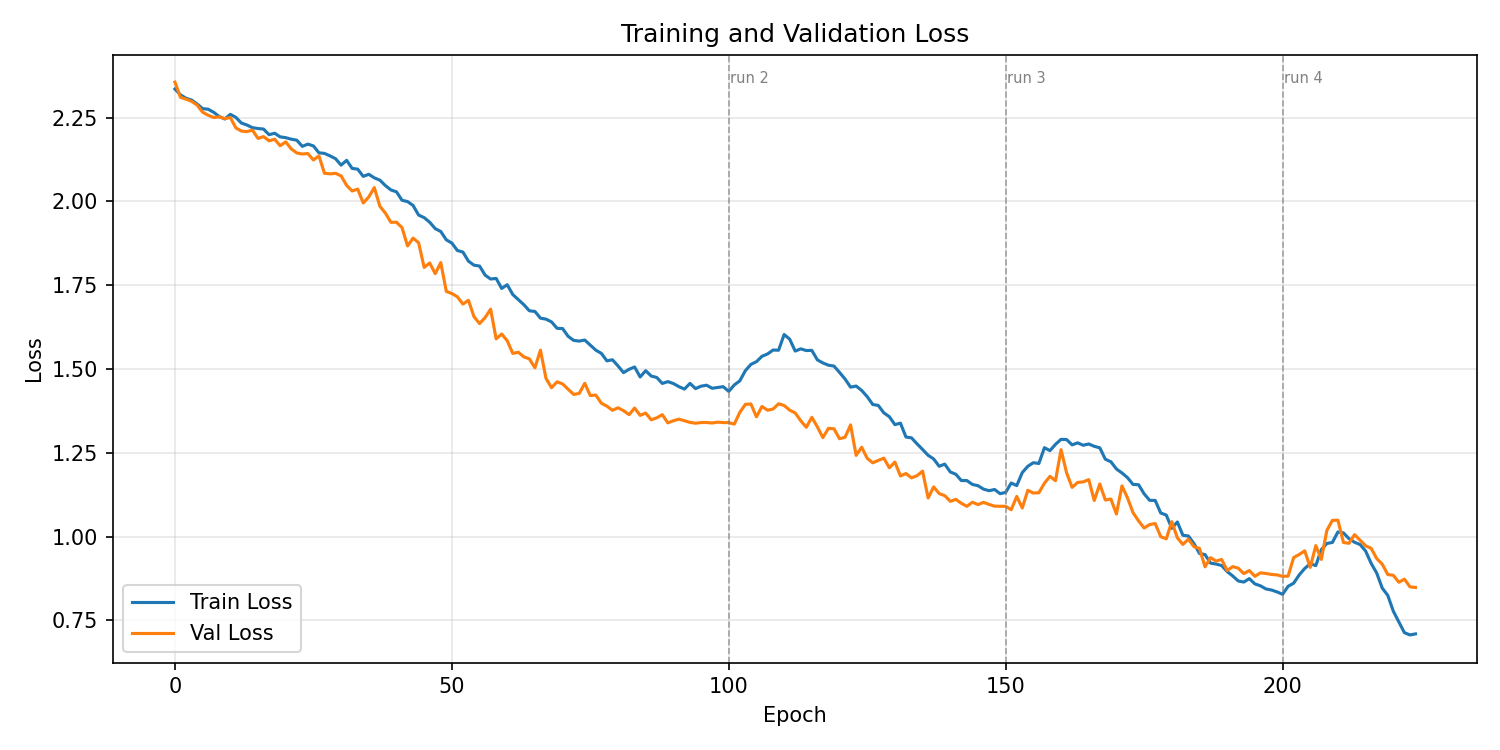
\includegraphics[width=0.5\textwidth]{figs/loss_curve.png}
  \caption{Loss over time with multiple restarted runs}
\end{figure}

Notice that we seem to do better on the validation set for a prolonged period, due to the augmentations encouraging robust generalization, until model performance saturates with training loss and accuracy approaching their validation counterparts, where I decide to stop training.

In every run, the model was trained using the AdamW optimizer with an initial learning rate of $3 \times 10^{-4}$ and weight decay set to $0.1$. A batch size of 128 was used. A cosine learning rate scheduler was used in all epochs, with $10$ warm-up epochs where the learning rate was linearly increased from 0 to $\text{lr}_\text{base} = 10^{-3}$, after which it decayed to $\text{lr}_\text{min} = 10^{-5} \approx 0$ following the function \begin{equation}
    \text{lr} = \text{lr}_\text{min} + (\text{lr}_\text{base} - \text{lr}_\text{min})\cdot 0.5 (1 + \cos (p_T))
\end{equation}
where $p_T$ represents the fraction of completed epochs after warmup. 

It was important to use warmups during each restart after each mini-run was complete, since there was no accumulated gradient information for momentum. 

Unlike in the CNN, model performance tended to climb linearly after escaping an initial low-quality parameter region which was stuck around 10\% accuracy.

I additionally tested the model without SPT or LSA, which are two architectural choices we introduce, over a simple 100-epoch run with learning rate decay. This stalls at 64.839\% validation accuracy. 

\begin{figure}[H]
  \centering
  
\includegraphics[width=0.9\textwidth]{figs/loss_acc_lr.png}
  \caption{Model over 100 epochs without SPT or LSA. Robust generalization is achieved but model performance saturates.}
\end{figure}

I found all setups to be highly sensitive to the choice of learning rate. My initial setups did not work for a long period with learning rates of $6 \times 10^{-4}$ and above, with a lot of my testing using $1 \times 10^{-3}$ due to that being succesful in my previous approach. I speculate this is to that choice of LR being too high initially, which causes the parameters to bounce around a tricky optimization region. I finally concluded this since there were typically gains during the first half of the warmup period but not after, and the longer I made the warmup period, the better the model's accuracy before stalling, which suggested that the lower learning rates were helpful. Due to time constraints, I was unfortunately not able to run a comprehensive study of learning rates, especially since it was very difficult with a ViT to quickly evaluate the quality of a setup, unlike a CNN.

More details on my architecture and optimization choices are in the next section.


\section{Model architecture}\label{sec:model}
\subsection{Interpretation}\label{sec:model-interpretation}
The full output of \texttt{print(model)} for the vanilla configuration is given in \autoref{sec:output-of-print-model}. I describe each component below. Note that we use SPT and LSA following \cite{lee2021vision}.

\begin{enumerate}
    \item \textbf{Patch embedding} (\texttt{patch\_embed: PatchEmbedding}). A single strided $8\times 8$ convolution maps the $128\times 128$ RGB image to a sequence of $N = (128/8)^2 = 256$ patch tokens, each of dimension $d = 192$. This layer plays an analogous role to the stem of a CNN: it discretises the continuous image into a fixed vocabulary of patch tokens that the transformer can process. With the SPT variant (\texttt{ShiftedPatchTokenization}), four diagonally-shifted copies of the image are concatenated channel-wise before patching (15 input channels instead of 3), so the projection becomes a \texttt{Linear(960, 192)} followed by a \texttt{LayerNorm}; this enlarges the effective receptive field of each token at embedding time without changing $N$.

    \item \textbf{CLS token and positional embedding} (\texttt{cls\_token}, \texttt{pos\_embed}, \texttt{pos\_drop}). A single learnable \texttt{[CLS]} vector of dimension 192 is prepended to the 256 patch tokens, giving a sequence of length 257. A learnable positional embedding of the same shape is added element-wise to encode spatial structure (transformers are otherwise permutation-invariant). \texttt{pos\_drop} is a dropout layer applied after embedding; it is disabled (p=0) in the final run but retained for completeness.

    \item \textbf{Transformer blocks} (\texttt{blocks: ModuleList}, 12 $\times$ \texttt{TransformerBlock}). The core of the model. Each block follows the Pre-LayerNorm DeiT convention:
    \[
      x \leftarrow x + \text{DropPath}(\text{Attn}(\text{LN}_1(x))), \quad
      x \leftarrow x + \text{DropPath}(\text{MLP}(\text{LN}_2(x))).
    \]
    \begin{itemize}
        \item \texttt{norm1} / \texttt{norm2}: \texttt{LayerNorm((192,))} — normalise each token's feature vector independently before each sub-layer, stabilising training and removing the need for careful learning-rate tuning.
        \item \texttt{attn: Attention} — multi-head self-attention with 3 heads (head dimension $= 192/3 = 64$). The \texttt{qkv} linear layer projects each token to queries, keys, and values simultaneously ($192 \to 576$); scaled dot-product attention is computed in parallel across heads; the \texttt{proj} linear maps the concatenated heads back to 192. This allows every token to aggregate information from all other tokens, including the \texttt{[CLS]} token, in $O(N^2)$ time. With LSA enabled, a learnable per-head temperature scalar replaces the fixed $1/\sqrt{d_\text{head}}$ scaling, and a diagonal mask prevents self-attention.
        \item \texttt{mlp: MLP} — a two-layer position-wise feed-forward network with hidden dimension $192 \times 4 = 768$, GELU activation, and dropout. This introduces non-linearity and per-token feature transformation independent of other tokens.
        \item \texttt{drop\_path: StochasticDepth} — randomly drops entire residual branches during training with linearly increasing probability (0 for block 0, up to 0.1 for block 11). Block 0 shows \texttt{Identity()} because its drop probability is 0; blocks 1–11 show \texttt{StochasticDepth()}.
    \end{itemize}

    \item \textbf{Final layer norm} (\texttt{norm: LayerNorm((192,))}). Applied to the full token sequence after all 12 blocks. This normalises representations before the classification head.

    \item \textbf{Classification head} (\texttt{head: Linear(in\_features=192, out\_features=10)}). A linear layer that maps only the \texttt{[CLS]} token's representation to 10 class logits. This is the \emph{only component directly responsible for classification}: it aggregates the global context accumulated by the \texttt{[CLS]} token across all 12 attention layers into a single prediction.
\end{enumerate}

\textbf{Low-level vs.\ high-level features.} Unlike CNNs, transformers do not have a strict hierarchy of receptive fields imposed by convolution strides. I speculate that early blocks (0--3) encode local, low-level structure: individual patch tokens attend primarily to spatially proximate neighbors, forming representations analogous to edge detectors. Intermediate blocks (4--8) build mid-level features as tokens begin to integrate information across larger spatial extents. Later blocks (9--11) are where the \texttt{[CLS]} token aggregates global semantic information — by block 11, the \texttt{[CLS]} token has attended, through successive rounds of self-attention, to every patch in the image, producing a holistic digit representation. The classification head reads from this globally integrated \texttt{[CLS]} embedding to produce final logits.

\subsection{Model capacity analysis}\label{sec:model-capacity}

The base DeiT-tiny model contains \textbf{5,427,274 parameters}. \autoref{tab:param-count} gives a component-by-component breakdown. Note that for a linear layer $\mathbb{R}^{m} \to \mathbb{R}^{n}$ the parameter count is $mn + n$.

\begin{table}[H]
\centering
\small
\begin{tabular}{lll}
\toprule
\textbf{Component} & \textbf{Formula} & \textbf{Count} \\
\midrule
Patch embedding \texttt{Conv2d(3, 192, 8, 8)} & $3 \times 192 \times 8^2 + 192$ & $37{,}056$ \\
CLS token & $192$ & $192$ \\
Positional embedding ($257 \times 192$) & $257 \times 192$ & $49{,}344$ \\
\midrule
\emph{Per TransformerBlock:} & & \\
\quad QKV projection \texttt{Linear(192, 576)} & $192 \times 576 + 576$ & $111{,}168$ \\
\quad Output projection \texttt{Linear(192, 192)} & $192 \times 192 + 192$ & $37{,}056$ \\
\quad MLP fc1 \texttt{Linear(192, 768)} & $192 \times 768 + 768$ & $148{,}224$ \\
\quad MLP fc2 \texttt{Linear(768, 192)} & $768 \times 192 + 192$ & $147{,}648$ \\
\quad Two LayerNorms \texttt{LN(192)} $\times$ 2 & $2 \times 2 \times 192$ & $768$ \\
\quad \emph{Block subtotal} & & \emph{$444{,}864$} \\
\midrule
12 TransformerBlocks & $12 \times 444{,}864$ & $5{,}338{,}368$ \\
\midrule
Final LayerNorm \texttt{LN(192)} & $2 \times 192$ & $384$ \\
CLS head \texttt{Linear(192, 10)} & $192 \times 10 + 10$ & $1{,}930$ \\
\midrule
\textbf{Total} & & $\mathbf{5{,}427{,}274}$ \\
\bottomrule
\end{tabular}
\caption{Parameter count for each component of the base DeiT-tiny model ($d=192$, 12 blocks, 3 heads, patch size 8, image size $128\times128$).}
\label{tab:param-count}
\end{table}

The 12 transformer blocks dominate, contributing 98.4\% of all parameters ($5{,}338{,}368$ of $5{,}427{,}274$). Within each block, the MLP sub-layer is the largest component (295,872 params, 66\%) because its hidden dimension is $4\times$ the embedding dimension; the attention sub-layer (148,224 params, 33\%) is smaller.

\textbf{Effect of architectural extensions.} SPT and LSA each add a modest number of additional parameters, summarised in \autoref{tab:variant-params}. SPT replaces the patch convolution with \texttt{Linear(960, 192)} plus a \texttt{LayerNorm}, increasing the patch-embedding count from 37,056 to 184,896 (+147,840). LSA adds one learnable temperature scalar per head per block ($12 \times 3 = 36$ parameters), a negligible change. In all cases the transformer blocks themselves are unchanged.

\begin{table}[H]
\centering
\small
\begin{tabular}{lrr}
\toprule
\textbf{Configuration} & \textbf{Parameters} & \textbf{$\Delta$ vs.\ base} \\
\midrule
Base (no SPT / LSA) & $5{,}427{,}274$ & --- \\
SPT only & $5{,}575{,}114$ & $+147{,}840$ \\
LSA only & $5{,}427{,}310$ & $+36$ \\
SPT + LSA (final model) & $5{,}575{,}150$ & $+147{,}876$ \\
\bottomrule
\end{tabular}
\caption{Total trainable parameter counts for the model configurations evaluated in this project.}
\label{tab:variant-params}
\end{table}

\textbf{Could the model have been smaller or larger?} The DeiT-tiny configuration (5.4M params) is already near the lower end of practical ViT scales. Given that our training set contains only $\sim 10^4$ unique images (even with repeated augmentation), a smaller model — e.g.\ fewer blocks or a narrower embedding — might have reduced overfitting risk; however, with aggressive augmentation and stochastic depth, overfitting was not observed to be severe in practice. Scaling up to DeiT-small (22M params, $d=384$, 6 heads) or DeiT-base (86M, $d=768$, 12 heads) would likely improve representational capacity, but at significantly higher memory and compute cost, and the gain may be limited by data quantity rather than model capacity.

\newpage
\appendix
\section{Augmentations used}

\begin{figure}[p]
\centering

% Images 1-10
\begin{subfigure}{\textwidth}
\begin{minipage}{0.75\textwidth}

\includegraphics[width=\linewidth]{figs/augmentation_examples/01_original.png}
\end{minipage}\hfill
\begin{minipage}{0.23\textwidth}
\caption{Original}
\end{minipage}
\end{subfigure}

\begin{subfigure}{\textwidth}
\begin{minipage}{0.75\textwidth}

\includegraphics[width=\linewidth]{figs/augmentation_examples/02_rand_augment.png}
\end{minipage}\hfill
\begin{minipage}{0.23\textwidth}
\caption{Random augmentation}
\end{minipage}
\end{subfigure}

\begin{subfigure}{\textwidth}
\begin{minipage}{0.75\textwidth}

\includegraphics[width=\linewidth]{figs/augmentation_examples/03_elastic_transform.png}
\end{minipage}\hfill
\begin{minipage}{0.23\textwidth}
\caption{Elastic transform}
\end{minipage}
\end{subfigure}

\begin{subfigure}{\textwidth}
\begin{minipage}{0.75\textwidth}
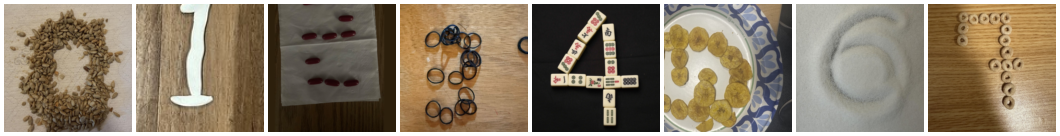
\includegraphics[width=\linewidth]{figs/augmentation_examples/04_random_resized_crop.png}
\end{minipage}\hfill
\begin{minipage}{0.23\textwidth}
\caption{Random resized crop}
\end{minipage}
\end{subfigure}

\begin{subfigure}{\textwidth}
\begin{minipage}{0.75\textwidth}
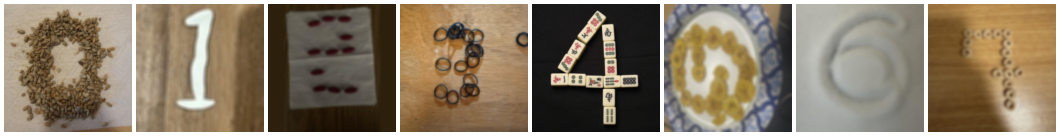
\includegraphics[width=\linewidth]{figs/augmentation_examples/05_gaussian_blur.png}
\end{minipage}\hfill
\begin{minipage}{0.23\textwidth}
\caption{Gaussian Blur}
\end{minipage}
\end{subfigure}

\begin{subfigure}{\textwidth}
\begin{minipage}{0.75\textwidth}
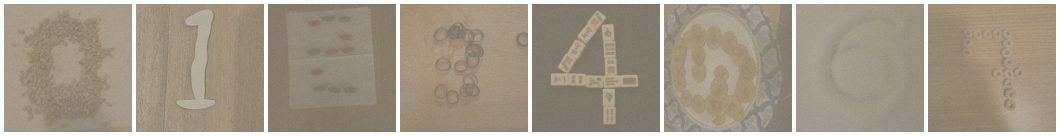
\includegraphics[width=\linewidth]{figs/augmentation_examples/06_gaussian_noise.png}
\end{minipage}\hfill
\begin{minipage}{0.23\textwidth}
\caption{Gaussian noise}
\end{minipage}
\end{subfigure}

\begin{subfigure}{\textwidth}
\begin{minipage}{0.75\textwidth}
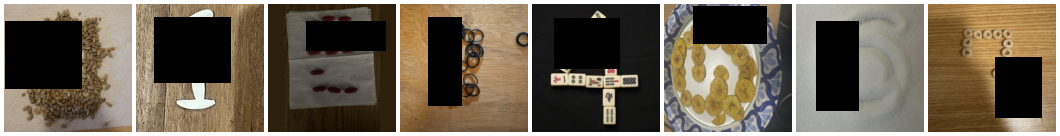
\includegraphics[width=\linewidth]{figs/augmentation_examples/07_random_erasing.png}
\end{minipage}\hfill
\begin{minipage}{0.23\textwidth}
\caption{Random erasing}
\end{minipage}
\end{subfigure}


\begin{subfigure}{\textwidth}
\begin{minipage}{0.75\textwidth}
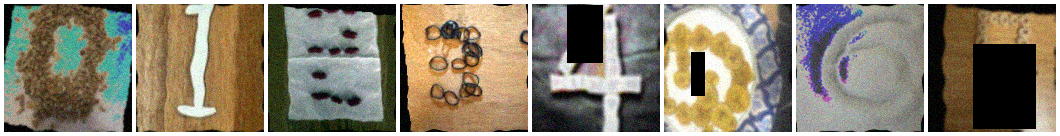
\includegraphics[width=\linewidth]{figs/augmentation_examples/08_full_pipeline.png}
\end{minipage}\hfill
\begin{minipage}{0.23\textwidth}
\caption{Full pipeline}
\end{minipage}
\end{subfigure}

\caption{Augmentation transforms applied to example images}
\label{fig:augmentations}
\end{figure}



\section{Output of \texttt{print(model)}}\label{sec:output-of-print-model}
\begin{verbatim}
VisionTransformer(
  (patch_embed): PatchEmbedding(
    (proj): Conv2d(3, 192, kernel_size=(8, 8), stride=(8, 8))
  )
  (pos_drop): Dropout(p=0.0, inplace=False)
  (blocks): ModuleList(
    (0): TransformerBlock(
      (norm1): LayerNorm((192,), eps=1e-05, elementwise_affine=True)
      (attn): Attention(
        (qkv): Linear(in_features=192, out_features=576, bias=True)
        (proj): Linear(in_features=192, out_features=192, bias=True)
        (attn_drop): Dropout(p=0.0, inplace=False)
      )
      (norm2): LayerNorm((192,), eps=1e-05, elementwise_affine=True)
      (mlp): MLP(
        (net): Sequential(
          (0): Linear(in_features=192, out_features=768, bias=True)
          (1): GELU(approximate='none')
          (2): Dropout(p=0.0, inplace=False)
          (3): Linear(in_features=768, out_features=192, bias=True)
          (4): Dropout(p=0.0, inplace=False)
        )
      )
      (drop_path): Identity()
    )
    (1-11): 11 x TransformerBlock(
      (norm1): LayerNorm((192,), eps=1e-05, elementwise_affine=True)
      (attn): Attention(
        (qkv): Linear(in_features=192, out_features=576, bias=True)
        (proj): Linear(in_features=192, out_features=192, bias=True)
        (attn_drop): Dropout(p=0.0, inplace=False)
      )
      (norm2): LayerNorm((192,), eps=1e-05, elementwise_affine=True)
      (mlp): MLP(
        (net): Sequential(
          (0): Linear(in_features=192, out_features=768, bias=True)
          (1): GELU(approximate='none')
          (2): Dropout(p=0.0, inplace=False)
          (3): Linear(in_features=768, out_features=192, bias=True)
          (4): Dropout(p=0.0, inplace=False)
        )
      )
      (drop_path): StochasticDepth()
    )
  )
  (norm): LayerNorm((192,), eps=1e-05, elementwise_affine=True)
  (head): Linear(in_features=192, out_features=10, bias=True)
  (dist_head): Linear(in_features=192, out_features=10, bias=True)
)
spt=False lsa=False: 5,429,204 params (5.43M)
  inference output: torch.Size([2, 10])
  train cls_out: torch.Size([2, 10]), dist_out: None
VisionTransformer(
  (patch_embed): ShiftedPatchTokenization(
    (proj): Linear(in_features=960, out_features=192, bias=True)
    (norm): LayerNorm((192,), eps=1e-05, elementwise_affine=True)
  )
  (pos_drop): Dropout(p=0.0, inplace=False)
  (blocks): ModuleList(
    (0): TransformerBlock(
      (norm1): LayerNorm((192,), eps=1e-05, elementwise_affine=True)
      (attn): Attention(
        (qkv): Linear(in_features=192, out_features=576, bias=True)
        (proj): Linear(in_features=192, out_features=192, bias=True)
        (attn_drop): Dropout(p=0.0, inplace=False)
      )
      (norm2): LayerNorm((192,), eps=1e-05, elementwise_affine=True)
      (mlp): MLP(
        (net): Sequential(
          (0): Linear(in_features=192, out_features=768, bias=True)
          (1): GELU(approximate='none')
          (2): Dropout(p=0.0, inplace=False)
          (3): Linear(in_features=768, out_features=192, bias=True)
          (4): Dropout(p=0.0, inplace=False)
        )
      )
      (drop_path): Identity()
    )
    (1-11): 11 x TransformerBlock(
      (norm1): LayerNorm((192,), eps=1e-05, elementwise_affine=True)
      (attn): Attention(
        (qkv): Linear(in_features=192, out_features=576, bias=True)
        (proj): Linear(in_features=192, out_features=192, bias=True)
        (attn_drop): Dropout(p=0.0, inplace=False)
      )
      (norm2): LayerNorm((192,), eps=1e-05, elementwise_affine=True)
      (mlp): MLP(
        (net): Sequential(
          (0): Linear(in_features=192, out_features=768, bias=True)
          (1): GELU(approximate='none')
          (2): Dropout(p=0.0, inplace=False)
          (3): Linear(in_features=768, out_features=192, bias=True)
          (4): Dropout(p=0.0, inplace=False)
        )
      )
      (drop_path): StochasticDepth()
    )
  )
  (norm): LayerNorm((192,), eps=1e-05, elementwise_affine=True)
  (head): Linear(in_features=192, out_features=10, bias=True)
  (dist_head): Linear(in_features=192, out_features=10, bias=True)
)
spt=True lsa=False: 5,577,044 params (5.58M)
  inference output: torch.Size([2, 10])
  train cls_out: torch.Size([2, 10]), dist_out: None
VisionTransformer(
  (patch_embed): PatchEmbedding(
    (proj): Conv2d(3, 192, kernel_size=(8, 8), stride=(8, 8))
  )
  (pos_drop): Dropout(p=0.0, inplace=False)
  (blocks): ModuleList(
    (0): TransformerBlock(
      (norm1): LayerNorm((192,), eps=1e-05, elementwise_affine=True)
      (attn): Attention(
        (qkv): Linear(in_features=192, out_features=576, bias=True)
        (proj): Linear(in_features=192, out_features=192, bias=True)
        (attn_drop): Dropout(p=0.0, inplace=False)
      )
      (norm2): LayerNorm((192,), eps=1e-05, elementwise_affine=True)
      (mlp): MLP(
        (net): Sequential(
          (0): Linear(in_features=192, out_features=768, bias=True)
          (1): GELU(approximate='none')
          (2): Dropout(p=0.0, inplace=False)
          (3): Linear(in_features=768, out_features=192, bias=True)
          (4): Dropout(p=0.0, inplace=False)
        )
      )
      (drop_path): Identity()
    )
    (1-11): 11 x TransformerBlock(
      (norm1): LayerNorm((192,), eps=1e-05, elementwise_affine=True)
      (attn): Attention(
        (qkv): Linear(in_features=192, out_features=576, bias=True)
        (proj): Linear(in_features=192, out_features=192, bias=True)
        (attn_drop): Dropout(p=0.0, inplace=False)
      )
      (norm2): LayerNorm((192,), eps=1e-05, elementwise_affine=True)
      (mlp): MLP(
        (net): Sequential(
          (0): Linear(in_features=192, out_features=768, bias=True)
          (1): GELU(approximate='none')
          (2): Dropout(p=0.0, inplace=False)
          (3): Linear(in_features=768, out_features=192, bias=True)
          (4): Dropout(p=0.0, inplace=False)
        )
      )
      (drop_path): StochasticDepth()
    )
  )
  (norm): LayerNorm((192,), eps=1e-05, elementwise_affine=True)
  (head): Linear(in_features=192, out_features=10, bias=True)
  (dist_head): Linear(in_features=192, out_features=10, bias=True)
)
spt=False lsa=True: 5,429,240 params (5.43M)
  inference output: torch.Size([2, 10])
  train cls_out: torch.Size([2, 10]), dist_out: None
VisionTransformer(
  (patch_embed): ShiftedPatchTokenization(
    (proj): Linear(in_features=960, out_features=192, bias=True)
    (norm): LayerNorm((192,), eps=1e-05, elementwise_affine=True)
  )
  (pos_drop): Dropout(p=0.0, inplace=False)
  (blocks): ModuleList(
    (0): TransformerBlock(
      (norm1): LayerNorm((192,), eps=1e-05, elementwise_affine=True)
      (attn): Attention(
        (qkv): Linear(in_features=192, out_features=576, bias=True)
        (proj): Linear(in_features=192, out_features=192, bias=True)
        (attn_drop): Dropout(p=0.0, inplace=False)
      )
      (norm2): LayerNorm((192,), eps=1e-05, elementwise_affine=True)
      (mlp): MLP(
        (net): Sequential(
          (0): Linear(in_features=192, out_features=768, bias=True)
          (1): GELU(approximate='none')
          (2): Dropout(p=0.0, inplace=False)
          (3): Linear(in_features=768, out_features=192, bias=True)
          (4): Dropout(p=0.0, inplace=False)
        )
      )
      (drop_path): Identity()
    )
    (1-11): 11 x TransformerBlock(
      (norm1): LayerNorm((192,), eps=1e-05, elementwise_affine=True)
      (attn): Attention(
        (qkv): Linear(in_features=192, out_features=576, bias=True)
        (proj): Linear(in_features=192, out_features=192, bias=True)
        (attn_drop): Dropout(p=0.0, inplace=False)
      )
      (norm2): LayerNorm((192,), eps=1e-05, elementwise_affine=True)
      (mlp): MLP(
        (net): Sequential(
          (0): Linear(in_features=192, out_features=768, bias=True)
          (1): GELU(approximate='none')
          (2): Dropout(p=0.0, inplace=False)
          (3): Linear(in_features=768, out_features=192, bias=True)
          (4): Dropout(p=0.0, inplace=False)
        )
      )
      (drop_path): StochasticDepth()
    )
  )
  (norm): LayerNorm((192,), eps=1e-05, elementwise_affine=True)
  (head): Linear(in_features=192, out_features=10, bias=True)
  (dist_head): Linear(in_features=192, out_features=10, bias=True)
)
spt=True lsa=True: 5,577,080 params (5.58M)
  inference output: torch.Size([2, 10])
  train cls_out: torch.Size([2, 10]), dist_out: None
\end{verbatim}


\section{AI Usage}\label{sec:ai-use}

I used Claude code to assist in the implementation of this project, particularly setting up the full pipeline on top of the basic model and data setup, adding visualization and adding additional studies once the basic pipeline was in place. I started off by providing it a markdown file describing my plan, which I had prepared using Claude (web version). After this point, I used it to iteratively refine and change my codebase. I list my prompts below.

Prompts for Claude web:
\begin{enumerate}
    \item For a class, I need to work on a ViT classifier of extremely adversarial data in an MNIST-style digit classification setting. Project 3 is an extension of project 2, using a ViT instead of a CNn.

I'm attaching my report for project 2 and the guidelines for project 3. Digest and understand the nature of this setting. I will then ask you more questions.

\item Let's think through ideas on how to improve performance.

I'm thinking we want to keep all my augmentations from the CNN project, and more - find more augmentations that are likely to work and are easy to implement (eg in the torchvision library) and justify why they would be a good idea for ViTs.

I'm leaning towards aggressively scaling up my synthetic data. Analyze this idea and critique it if it isn't good. Notice the way I'm generating it as per my description in project 2.

Provide further analysis on ways this project might be different from and require changes rlative to project 2


\item (I found the DeiT-tiny paper and linked it) Analyze the extent to which this would work here, considering I only have a pretrained Resnet-18 model available. If it would work, consider what architectural changes would have to be made. It seems like they propose:
1. Soft distillation loss
2. Hard distillation loss
3. Any loss with a learnable distillation token
COrrect my understanding if it's wrong

Ideally, for my project and report, I'll try to make minimal changes to the base vit architecture to account for distillation - so, for example, just add in the distillation token. this makes it nice for comparison / analysis

\item Can you give some intuition for why hard distillation works? Why is it better than just training on ground truth?

\item Do further literature review of ideas for VITs in sparse data regimes.

\item What are some other general hacks for making training more efficient?
* My heuristic is that larger batches --> better for transformer. Is this correct? I'll scale up as much as possible
* Should I use the muon optimizer instead of AdamW?

\item \textit{I wrote a markdown file of instructions and uploaded them} Review these instructions for a coding agent - are they clear and comprehensive? Are there important other ideas I should include?

Markdown file given to Claude code: \begin{verbatim}
  You are in a directory which contains code for project 2 and project 3. Project 2 involved training a CNN on 'adversarial' MNIST data - 10k images intentionally constructed by many humans to create aderversarial examples for a digit classifier. 

Project 2 used Resnet-18 with an aggressive augmentation pipeline to achieve 95% accuracy. The final model is stored in project2/checkpoints/run10_final_9k/best_model.pt. We now have to use a ViT for project 3.


I will give you a list of features I want to implement. I will then give instructions on directory setup.

## Features


Augmentations: for the CNN, we had 
```
def get_train_transform(img_size: int = 128):
    return transforms.Compose([
        transforms.RandomResizedCrop(img_size, scale=(0.7, 1.0), ratio=(0.75, 1.33)),
        transforms.RandomRotation(20),
        transforms.RandomPerspective(distortion_scale=0.2, p=0.5),
        transforms.ColorJitter(brightness=0.4, contrast=0.4, saturation=0.4, hue=0.1),
        transforms.GaussianBlur(kernel_size=5, sigma=(0.1, 2.0)),
        transforms.ToTensor(),
        transforms.Lambda(lambda x: x + torch.randn_like(x) * 0.05),
        transforms.RandomErasing(p=0.25, scale=(0.02, 0.15)),
        transforms.Normalize(mean=[0.485, 0.456, 0.406],
                             std=[0.229, 0.224, 0.225]),
    ])
```

We're going to change this to:
```
def get_train_transform(img_size: int = 128):
    return transforms.Compose([
        transforms.RandomResizedCrop(img_size, scale=(0.7, 1.0), ratio=(0.75, 1.33)),
        transforms.RandAugment(num_ops=2, magnitude=9),
        transforms.ElasticTransform(alpha=50.0, sigma=5.0),
        transforms.GaussianBlur(kernel_size=5, sigma=(0.1, 2.0)),
        transforms.ToTensor(),
        transforms.Lambda(lambda x: x + torch.randn_like(x) * 0.05),
        transforms.RandomErasing(p=0.25, scale=(0.02, 0.33)),  # CutOut is just larger-scale erasing
        transforms.Normalize(mean=[0.485, 0.456, 0.406],
                             std=[0.229, 0.224, 0.225]),
    ])
```

Remember val transform should be just
```
    """Deterministic transform for validation."""
    return transforms.Compose([
        transforms.Resize((img_size, img_size)),
        transforms.ToTensor(),
        transforms.Normalize(mean=[0.485, 0.456, 0.406],
                             std=[0.229, 0.224, 0.225]),
    ])
```

We're additionally going to implement _repeated augmentation_: in every epoch, sample each image multiple times with different augmentation draws, rather than once, so the model sees far more variation per unique sample. Do this by repeating each index in the dataset N times per epoch via a custom sampler. N should be 3 by default.

Additionally apply, dependent on a CLI arg, Locality Self-Attention, which contains:
1. diagonal masking, which prevents each token from attending to itself (since self-similarity is trivially high and dominates attention scores, masking it forces the model to attend to other patches)
2. learnable temperature scaling of the softmax, which allows the model to learn how sharply or diffusely to distribute attention rather than fixing it with the standard d normalization.

Apply, dependent on a CLI arg, Shifted Patch Tokenization. This involves taking the image, creating four diagonal shifts of it (up-left, up-right, down-left, down-right), concatenating these shifted copies channel-wise with the original, and then extracting patches from this enriched representation. The effect is that each patch token now contains information about its immediate neighbors at embedding time, effectively increasing the receptive field without changing the attention mechanism. Note that this means that SPT does not change N. we still have the same number of patches after tokenization. What changes is the input dimensionality to the linear patch embedding layer: instead of projecting a patch of shape (3 x  P x  P), you're projecting a concatenated patch of shape (3x 5 x  P x  P) — the original plus four shifted copies, each with 3 channels.

Let's keep synthetic data to 3k images in default CLI args. 

### Training strategy

Learning rate warmup: 15 warmup epochs by default for 50 training epochs. Set this as an arg
Regularization:
- Stochastic depth - randomly drop entire transformer blocks. Set to 0.1


### Distillation approaches

We have a pretrained CNN model which achieves 95% accuracy in project2/checkpoints/run10_final_9k/best_model.pt. We follow approaches provided by https://arxiv.org/pdf/2012.12877 for distilling a CNN to a ViT


1. Soft distillation
Loss = (1 - \lambda) * cross entropy loss of student against ground truth+ lambda * tau^2 KL (softmax(student logics / tau), softmax(teacher logits / tau))    
where tau is temperature

2. Hard distillation
0.5 * cross entropy loss of student against ground truth + 0.5* cross entropy loss against hard decision of teacher 

Distillation token:
> We now focus on our proposal, which is illustrated in Figure 2. We add a new token, the distillation token, to the initial embeddings (patches and class token). Our distillation token is used similarly as the class token: it interacts with other embeddings through self-attention, and is output by the network after the last layer. Its target objective is given by the distillation component of the loss. The distillation embedding allows our model to learn from the output of the teacher, as in a regular distillation, while remaining complementary to the class embedding.
So when using the distillation token with hard distillation, the loss is just 0.5 CE (CLS head output, true label) + 0.5 CE (distillation head output, teacher argmax)

We should design our training pipeline such that we can switch from:
1. No distillation loss
2. Soft distillation loss with lambda and tau as hyperparameters
3. Hard distillation loss 
4. Hard distillation loss with the distillation token


distillation token is only used with hard distillation

## Directory setup

I want to follow a similar setup as project2/.
`src`: contains
- dataset.py
- model.py
- train.py
- pipeline.py (for final submission to HF - look at project 2 as a reference)

In model.py, set up a skeleton for the ViT, but don't fill it in yet - I want to code up the blocks. Let's use DeiT-tiny for the skeleton, with depth=12, dim=192, heads=3, patch_size=16.

`src` also contains visualize_augmentations, visualize_embeddings, visualize_errors, visualize_pca, verify_pipeline.py. It should also contain generate_dashboard, generate_index. Look at the original ones and make whichever changes are necessary, but many should not be required.

A major change from project 2 is that I now want to do training in a notebook so I can use colab resources. I want to use the Visual Studio code extension for Colab: https://github.com/googlecolab/colab-vscode. But you're going to need to design this in a special way - for example, cloning the repository and pulling everything it needs from project 3. 

I want scripts / a notebook to be set up for the following experiments:
1. Run a vanilla ViT, with augmentations but without distillation, SPT, LSA. 
2. Ablation over soft distillation, hard distillation, hard distillation with distillation token. Set a reasonable set of parameters for tau and lambda considering our dataset size and model size (11M params for Resnet-18)
3. Ablation over vanilla + SPT, vanilla + LSA, vanilla + SPT + LSA
4. Final script which will contain all the things we want - for now, assume we add in SPT, LSA, hard distillation with distillation token
\end{verbatim}


\end{enumerate}

Prompts for Claude code:
\begin{enumerate}
  \item Wait, is this implementation of stochastic depth fine? it only drops residual branches. [Pasted text \#1 +21 lines]   
  \item  Change this to use 64x64 everywhere with a 8x8 patch size.  
  \item Make those changes to lr - drop it to 3e-4 and warmup epochs to just 5. The  
  weight decay fix isn't doing anything right now but there haven't been enough  
  epochs to tell            
  \item Refactor the repository to get rid of all parts where plot with the tex font in matplotlib - it fails on colab 
\end{enumerate}



\bibliographystyle{plainnat}
\bibliography{refs}

\end{document}